% !TEX root = twibop2.tex
\chapter{Decision Making}
\epigraph{Practical demands brought forth special scientific methods
  that can be collected under the heading ``operations research''. We
  shall use this term to mean the application of quantitative
  mathematical methods to justify decisions in every area of
  goal-oriented human activity.}  {E. S. Wentzel}

\section{These Difficult Decisions}

\txthead{Decision making under uncertain conditions.} We often have to make decisions when not all the information is
available and this uncertainty always decreases to some extent our
ability to decide. For example, where to go for a vacation or holiday?
This has worried me many times, since various uncertainties concerning
the weather, the hotel, the entertainment at the resort, and so on,
must be foreseen. We try and decide on the best variant from our
experience and the advice of our friends, and we often act ``by
inspiration''. This \redem{subjective} approach to decision making is
justifiable when the consequences involve ourselves and
relatives. However, there are many situations when a decision can
affect a large number of people and therefore requires a \redem{scientific}
and \redem{mathematically justifiable} approach rather than a
subjective one.


For instance, modern society cannot function without electricity,
stores of food, raw materials, etc. The stores are kept everywhere: at
factories, shops, hospitals, and garages. But how large should the
stores be in a particular case? It is clear that they should not be
too small, otherwise the function of the enterprise would be
interrupted. Neither should they also be too large because they cost
money to build and maintain: they would be dead stock. \redem{Store-keeping} is a problem of exceptional importance. It is so complicated because a decision must always be made in conditions of uncertainty.

\txthead{Two kinds of uncertainty.} How should we make decisions under conditions of uncertainty? First of
all, we should discover which factors are causing the uncertainty and
evaluate their nature. There are two kinds of uncertainty. The first
kind is due to factors which can be treated using the theory of
probability. These are either \redem{random variables} or \redem{random
  functions}, and they have statistical properties (for instance, the
expected value and variance), which are either known or can be
obtained over time. Uncertainty of this kind is called
\redem{probabilistic} or \redem{stochastic}. The second kind of
uncertainty is caused by unknown factors which are not random
variables (random functions) because the set of realizations of these
factors does not possess statistical stability and therefore the
notion of probability cannot be used. We shall call this uncertainty
``bad''.

``So'', the reader may say, ``it would seem that not every event that
cannot be predicted accurately is a random event.''

``Well, yes, in a way.'' Let me explain. In the preceding chapter we
discussed random events, random variables, and random functions.  I
repeatedly emphasized that there should always be \redem{statistical
  stability}, which is expressed in terms of probability. However,
there are events, which occur from time to time, that do not have any
statistical stability. The notion of probability is inapplicable to
such events, and therefore, the term ``random'' cannot be used here
too. For instance, we cannot assign a probability to the event of an
individual pupil getting an unsatisfactory mark in a concrete
subject. We cannot, even hypothetically, devise a set of uniform
trials that might yield the event as one outcome. There would be no
sense in conducting such a trial with a group of pupils because each
pupil has his or her own individual abilities and level of preparation
for the exam. The trials cannot be repeated with the same pupil
because he will obviously get better and better in the subject from
trial to trial. Similarly there is no way we can discuss the
probability of the outcome of a game between two equally matched chess
players. In all such situations, there can be no set of uniform
trials, and so there is no stability which can be expressed in terms
of a probability. We have ``bad'' uncertainty in all such situations.


I am afraid we do not consider the notion ``statistical stability'' and
often use expressions such as ``improbable'', ``probable'', ``most
probable'', and ``in all probability'' to refer to events that cannot be
assigned by any probability. We are apt to ascribe a probability to every
event even though it might not be predictable. This is why it became
necessary to refine the notion of probability early this century. This was
done by A.N. Kolmogorov when he developed an axiomatic definition
of probability.

\txthead{Options and the measure of effectiveness.} When we speak of
decision making, we assume that different patterns of behaviour are
possible.  They are called \redem{options}. Let me emphasize that in
the more important problems the number of options is very great. Let
$X$ be the set of options in a particular situation. A decision is
made when we select one option $x$ from this set. How do we determine
which option is the most preferable or the most efficient? A
quantitative criterion is needed to allow us to compare different
options in terms of their effectiveness. Let us call this criterion
the \redem{measure of effectiveness}. This measure is selected for each
particular \redem{purpose}, e.g., not to be late for school, to solve a
problem correctly and quickly, or to reach the cinema. A doctor wants
to find an efficient method of treating his patient. A factory manager
is responsible for the fulfilment of a production plan. The most
efficient option is the one that suits its purpose best.


Suppose we work in a shop and our target is to maximize the
receipts. We could choose profit as the measure of effectiveness and
strive to maximize this measure. The selection of the measure in this
example is evident. However, there are more complicated situations,
when several goals are pursued simultaneously, for example, we wish to
maximize profit, minimize the duration of the sales, and distribute the
goods to the greatest number of customers. In such cases we have to
have several measures of effectiveness; these problems are called
multi-criterial.

Let $W$ be a single measure of effectiveness. It would seem that our
task is now to find an option $x$ at which $W$ is at a maximum (or, the
other way round, at a minimum). However, we should remember that
decision making occurs under conditions of uncertainty. There are
unknown (random) factors (let us use $\xi$ to denote them), which influence
the end result and therefore affect the measure of effectiveness $W$. There
is also always a set of factors known beforehand (let us designate them
$\alpha$). Therefore the measure of effectiveness is dependent on three groups
of factors: known factors $\alpha$, unknown (random) factors $\xi$, and the
selected option $x$:
\begin{equation*}%
W= W(\alpha, \xi, x).
\end{equation*}
In the sales example, the $\alpha$ set is goods on sale, the available premises,
the season, etc. The $\xi$ factors include the number of customers per day
(it varies randomly from day to day), the time customers arrive (random
crowding is possible, which leads to long queues), the goods chosen by
the customers (the demand for a given commodity varies randomly in
time), etc.

Since the $\xi$, factors are random, the measure of effectiveness $W$ is
a random variable. Now, how is it possible to maximize (minimize)
a random variable? The answer quite clearly is that it is naturally
impossible. Whichever option $x$ is chosen, $W$ remains random, and it
cannot be maximized or minimized. This answer should not discourage
the reader. It is true that under conditions of uncertainty we cannot
maximize (minimize) the measure of effectiveness with a hundred per
cent probability. However, an adequate selection of an option is possible
with a reasonably large probability. This is where we should tackle the
techniques used in decision making under conditions of stochastic
uncertainty.

\txthead{Substitution of random factors by means.} The easiest
technique is merely to substitute the random factors $\xi$ by their
means. The result is that the problem becomes completely determined
and the measure of effectiveness $W$ can be calculated precisely. It
can, in particular, be either maximized or minimized. This technique
has been widely used to solve problems in physics and
technology. Almost every parameter encountered in these fields (e.g.,
temperature, potential difference, illuminance, pressure) is, strictly
speaking, a random variable. As a rule, we neglect the random nature
of physical parameters and use their mean values to solve the
problems.

The technique is justified if the deviation of a parameter from its
mean value is insignificant. However, it is not valid if the random factor
significantly affects the outcome. For instance, when organizing the jobs
in a motor-car repair shop, we may not neglect the randomness in the
way cars fail, or the random nature of the failures themselves, or the
random time needed to complete each repair operation. If we are
dealing with the noise arising in an electronic device, we cannot neglect
the random behaviour of electron flows. In these examples, the $\xi$ factors
must indeed be considered as random factors, we shall say they are
essentially random.

\txthead{Mean value optimization.} If the $\xi$ factors are essentially
random, we can use a technique called \redem{mean-value
  optimization}. What we do is to use the expected value $E (W)$ as the
measure of effectiveness, rather than the random variable $W$ and the
expected value is maximized or minimized.

Naturally, this approach does not resolve the uncertainty. The
effectiveness of an option $x$ for concrete values of random
parameters $\xi$ may be very different from the expected one. However,
using mean-value optimization means that we can be sure that after
many repeated operations we shall gain overall. It should be borne in
mind that mean-value optimization is only admissible when the gains of
repeated operations are \redem{totalled}, so that ``minuses'' in some
operations are compensated by the ``pluses'' in others. Mean-value
optimization would be justified should we be trying to increase the
profit obtained, for instance, in a sales department. The profit on
different days would be totalled, so that random ``unlucky'' days
would be compensated by the ``lucky'' days,

But here is another example. Suppose we consider the effectiveness of
the ambulance service in a large city. Let us select the elapsed time
between summoning help and the ambulance arriving as the measure of
effectiveness. It is desirable that this parameter be minimized. We cannot
apply mean-value optimization because if one patient waits too long for
a doctor, he or she is not compensated by the fact that another patient
received faster attention.

\txthead{Stochastic constraints.} Let us put forward an additional
demand.  Suppose we desire that the elapsed time $W$ till the arrival
of help after a call for an ambulance be less than some value
$W_{0}$. Since $W$ is a random variable, we cannot demand that the
inequality $W< W_{0}$ be always true, we can only demand that it be
true for some large probability, for instance, no less than 0.99. In
order to take this into account we delete from the $X$ set those
options $x$, for which the requirement is not satisfied. These
\redem{constraints} are called \redem{stochastic}.  Naturally, the use
of stochastic constraints noticeably complicates decision making.


\section{Random Processes with Discrete States}
A \redem{random} process can be thought of as the transition of a system from
one state to another occurring in a random fashion. We shall consider
random processes with \redem{discrete states} in this chapter and so our system
will be supposed to have a set of discrete states, either finite or infinite.
The random transitions of the system from one state to another are
assumed to take place \redem{instantaneously}.

\txthead{State graphs.} Random processes with discrete states can be
conveniently considered using a diagram called a \redem{state graph}. The
diagram shows the possible states a system may be in and indicates the
possible transitions using arrows.
 \begin{wrapfigure}[12]{O}{\mfwidth}
 \centering
 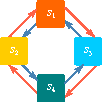
\includegraphics[width=0.9\linewidth]{figures/state-graph1.pdf}
\caption{A state graph for system with four states.}
\label{state-graph1}
 \end{wrapfigure}
 
Let us take an example. Suppose a system consists of two machine
tools, each of which produces identical products. If a tool fails its repair
is started immediately. Thus, our system has four states: $S_{1}$ both tools
are operating; $S_{2}$ the first tool is under repair after a failure while the
second is operating; $S_{3}$, the second tool is under repair while the first is
operating; $S_{4}$, both tools are being repaired.

The state graph is given in \figr{state-graph1}. The transitions
$S_{1} \to S_{2}, \,\, S_{1} \to S_{3}, \,\, S_{2} \to S_{4}$ and
$S_{3} \to S_{4}$ occur as a result of failures in the system. The
reverse transitions take place upon termination of the
repairs. Failures occur at unpredictable moments and the moments when
the repairs are terminated are also random. Therefore, the system's
transition from state to state is random.



 Note that the figure does not show transitions $S_{1} \to S_{4}$ and
 $S_{4} \to S_{1}$.  The former corresponds to the simultaneous
 failure of both tools and the latter to the simultaneous termination
 of repair of both tools. We shall assume that the probabilities of
 these events are zero.

 \txthead{Event arrival.} Suppose that we have a situation in which a
 \redem{stream of uniform events} follow each other at random moments. They
 may be telephoned orders for taxi, domestic appliances being switched
 on, the failures in the operation of a device, etc.

 \begin{figure}[!ht]
 \centering
 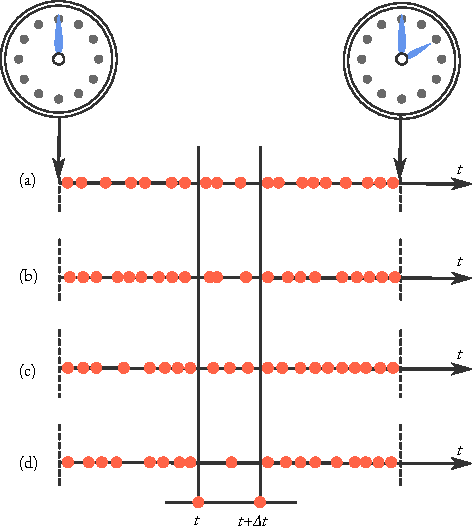
\includegraphics[width=0.85\tfwidth]{figures/event-arrival.pdf}
\caption{A record of taxi orders at a taxi depot.\label{event-arrival}}
 \end{figure}


 Suppose the dispatcher at a taxi depot records the time each taxi
 order is made over an interval of time, for instance, from 12 a.m. to
 2 p.m. We can show these moments as points on the time axis, and so
 the dispatcher might get the pattern illustrated in 
 \figr{event-arrival}~\drkgry{(a)}. This is the realization of the taxi-call arrivals  during that interval of time. Three more such realizations are shown
 in \figr{event-arrival}~\drkgry{(b)}, \drkgry{(c)}, and \drkgry{(d)}, and they are patterns recorded on different days. The moments when each taxi order is made
 in each realization are random. At the same time, the taxi-order arrivals possess statistical stability, that is, the total number of events in each interval of time varies only slightly from experiment to experiment
(from one arrival realization to another). We can see that the number of
events in the arrival realisations presented are 19, 20, 21, and 18.

In the preceding chapter, a random event in an experiment was an
outcome which has a definite probability. When we are considering
arrivals of events, we must have another meaning for the term
``event''.  There is no use speaking about the probability of an
outcome (event) because each event is uniform, i.e. indistinguishable
from the others. For instance, one taxi-order is a single event in a
stream and is indistinguishable from another event. Now let us
consider other probabilities, for instance, the probabilities that an
event will occur during a given interval of time (suppose, from $t$ to
$t + \Delta t$, as shown in the figure) exactly once, twice, thrice,
etc.

The notion of ``event arrival'' is applied to random processes in
systems with discrete states. It is assumed that the transitions of a
system from one state to another occur as a result of the effect of
event arrivals. Once an event arrives, the system instantaneously
changes state. For the state graph in \figr{state-graph1} transitions
$S_{1} \to S_{2}$ and $S_{3} \to S_{4}$ occur due to the arrival of
events corresponding to failures in the first tool, while transitions
$S_{1} \to S_{3}$ and $S_{2} \to S_{4}$ occur due to failures of the
second tool. The reverse transitions are caused by the arrival of
events corresponding to the ``terminations'' of repair: transitions
$S_{2} \to S_{1}$ and $S_{4} \to S_{3}$, are caused by the arrivals of
repair terminations of the first tool, and transitions
$S_{3} \to S_{1}$ and $S_{4} \to S_{2}$ to the arrivals of repair
terminations of the second tool.

The system transfers from state $S_{i}$ to state $S_{j}$ every time
the next event related to the transition arrives. The natural
conclusion is that the probability of transition $S_{i} \to S_{j}$ at
a definite moment in time $t$ should equal the probability of an event
arrival at this moment. There is no sense in speaking of the
probability of a transition at a concrete moment $t$. Like the
probability of any concrete value of a continuous random variable,
this probability is zero, and this result follows from the continuity
of time. It is therefore natural to discuss the probability of a
transition (the probability of an event arrival) occurring during the
interval of time from $t$ to $t+ \Delta t$, rather than its occurrence
at time $t$. Let us designate this probability $P_{ij}(t, \Delta
t)$. As $\Delta t$ tends to zero, we arrive at the notion of a
\redem{transition probability density} at time $t$, i.e. 
\begin{equation}%
\lambda_{j} (t) = \lim_{\Delta t \rightarrow 0} x =  \frac{P_{ij}\,(
  t, \Delta t)}{\Delta t}.
\label{eq-2.1}
\end{equation}
This is also called the \redem{arrival rate of events} causing the transition in
question.

In the general case, the arrival rate depends on time. However, it should
be remembered that the dependence of the arrival rate on time is
not related to the location of ``dense'' or ``rare'' arrival realisations. For
simplicity's sake, we shall assume that the transition probability density
and therefore the event arrival rate does not depend on time. i.e. we
shall consider \redem{steady-state} arrivals.


 \begin{wrapfigure}{O}{\mfwidth}%[h]
 \centering
 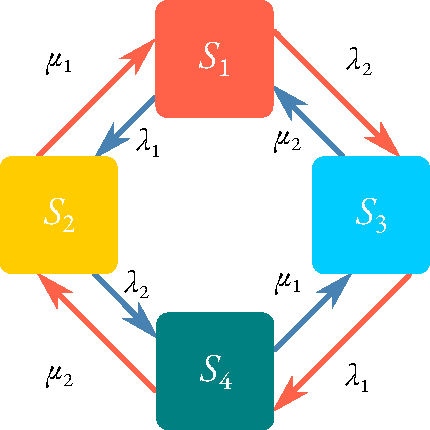
\includegraphics[width=0.9\linewidth]{figures/state-graph2.pdf}
\caption{A state graph for system with four states with arrival rates.
\label{state-graph2}}
 \end{wrapfigure}
 
\txthead{The Chapman-Kolmogorov equations for steady state.} Let us
use $p_{i}$ to denote the probability that a system is in state
$S_{i}$ (since our discussion is only for \redem{steady-state}
arrivals, the probabilities $p_{i}$, are independent of time), Let us
consider the system whose state graph is given in \figr{state-graph1}. Suppose $\lambda_{1}$ is the arrival rate for failures of the first tool and $\lambda_{2}$ that for the second tool; let $\mu_{1}$ be the arrival rate for repair terminations of the first tool and $\mu_{2}$ that for the second tool. We have labelled the state graph with the appropriate arrival rates, see \figr{state-graph2}.



 Suppose there are $N$ identical systems described by the state graph
 in \figr{state-graph2}. Let $N \gg 1$. The number of systems with
 state $S_{i}$, is $N p_{i}$ (this statement becomes more accurate the
 larger $N$ is). Let us consider a concrete state, say,
 $S_{1}$. Transitions are possible from this state to states $S_{2}$
and $S_{3}$ with probability $\lambda_{1} + \lambda_{2}$, per unit
time. (Under steady state, the probability density is the probability
for the finite time interval $\Delta t$ divided by $\Delta t$.)
Therefore, the number of departure: from state $S_{1}$, per unit time in
the considered set of systems is $N p_{ 1}\, (\lambda_{1}+\lambda_{2})$,
We can discern a general rule here: the number of transitions
$S_{i} \to S_{j}$ per unit time is the product of the number of
systems with state $S_{i}$ (the initial state) by the probability of
the transition per unit time, We have considered departures from state
$S_{1}$. The system arrives at this state from $S_{2}$ and $S_{3}$, The number
of arrivals at $S_{1}$ per unit time is $N p_{2} \, \mu_{1} + N p_{3}
\, \mu_{1}$. Since we are dealing
with steady states, the number of departures and arrivals for each
particular state should be balanced.  Therefore.  
\begin{equation*}%
N p_{ 1}(\lambda_{1}+\lambda_{2}) = N p_{2} \, \mu_{1} + N p_{3} \, \mu_{2}.
\end{equation*}
By setting up similar balances of arrivals and departures for each of
the four states and eliminating the common factor $N$ in the equations, we obtain the following equations for probabilities $p_{1}, \, p_{2},
\, p_{3}$ and $p_{4}$:
\begin{align*}%
\text{for state} \,\,  S_{1}: (\lambda_{1} + \lambda_{2}) \, p_{1} &
= \mu_{1} p_{2} + \mu_{2} p_{3}, \\
\text{for state} \,\,  S_{2}: (\lambda_{2} + \mu_{1}) \, p_{2} &
= \lambda_{1} p_{1} + \mu_{2} p_{4}, \\
\text{for state} \,\,  S_{3}: (\lambda_{1} + \mu_{2}) \, p_{3} &
= \lambda_{1} p_{1} + \mu_{1} p_{4}, \\
\text{for state} \,\,  S_{4}: (\mu_{1} + \mu_{2}) \, p_{4} &
= \lambda_{2} p_{2} + \lambda_{1} p_{3}. 
\end{align*}
It is easy to see that the fourth equation can be obtained by summing
the first three. Instead of this equation, let us use the equation
\begin{equation*}%
p_{1}+p_{2}+p_{3}+p_{4}= 1,
\end{equation*}
which means that the system must be in one of the four states.
Therefore, we have the following system of equations:
\begin{equation}%
\left.
\begin{split}
S_{1}: (\lambda_{1} + \lambda_{2}) \, p_{1} & = \mu_{1} p_{2} + \mu_{2} p_{3}, \\
S_{2}: (\lambda_{2} + \mu_{1}) \, p_{2} & = \lambda_{1} p_{1} + \mu_{2} p_{4}, \\
S_{3}: (\lambda_{1} + \mu_{2}) \, p_{3} & = \lambda_{2} p_{1} + \mu_{1} p_{4},  \\
p_{1} + p_{2} + p_{3} + p_{4} & = 1.
\end{split}
\right\}
\label{eq-2.2}
\end{equation}
These are the \redem{Chapman-Kolmogomv equations} for the system whose state
graph is shown in \figr{state-graph2}.

\txthead{Which innovation should be chosen?} Let us analyze a concrete
situation using equations \eqref{eq-2.2}. The state graph (see \figr{state-graph2})
corresponding to these equations describes a system which, we assumed,
consists of two machine tools each producing identical goods Suppose
the second tool is more modern an its output rate is twice that o the
first tool. The first tool generates (per unit time) an income of five
conventional units, while the second one generates one of ten units.
Regretfully, the second tool fails, on the average, twice as
frequently as does the first tool: hence $\lambda_{1} = 1$ and
$\lambda_{2} =2$. The arrival
rates for repair termination are assumed to be $u_{1} =2$ and $u_{2} =3$. Using
these arrival rates for failure and repair termination. let us rewrite
(\ref{eq-2.2}) thus 
\begin{equation*}
\left.
\begin{split}
3p_{1} & = 2p_{2} + 3p_{3}, \\
4p_{2} & = p_{1} + 3p_{4}, \\
4p_{3} & = 2p_{1} + 2p_{4}, \\
p_{1} +p_{2}&+p_{3}+p_{4}= 1.
\end{split}
\right\}
\end{equation*}
This system of equations can be solved to yield
$p_{1}= 0.4, \, p_{2}=0.2, \, p_{3} = 0.27$ and $p_{4} = 0.13$. This
means that, on the average, both tools operate simultaneously (state
$S_{1}$ in the figure) 40 per cent of the time, the first tool operates
while the second one is being repaired (state $S_{2}$) 20 per cent of
the time, the second tool operates while the first one is being
repaired (state $S_{3}$) 27 per cent of the time, and both tools are
simultaneously being repaired (state $S_{4}$) 13 per cent of the
time. It is easy to calculate the income this tool system generates
per unit time: $(5+10) \times 0.4+5 \times 0.2+10 \times 0.27 =9.7$
conventional units.

Suppose an innovation is suggested which would reduce the repair time of either the first or second tool by a factor of two. For technical reasons, we can only apply the innovation to one tool. Which tool should be chosen, the first or the second? Here is a concrete example of a practical situation when, using probability theory, we must justify our decision scientifically

Suppose we choose the first tool. Following the introduction of the
innovation, the arrival rate of its repair termination increases by a
factor of two, whence $u_{1} = 4$ (the other rates remain the same,
i. e. $\lambda_{1} = 1, \lambda_{2} = 2$ and $\mu_{2} =3$). Now
equations \eqref{eq-2.2} are 
\begin{equation*}
\left.
\begin{split}
3p_{1} & = 4p_{2} + 3p_{3}, \\
6p_{2} & = p_{1} + 3p_{4}, \\
4p_{3} & = 2p_{1} + 4p_{4}, \\
p_{1} +p_{2}&+p_{3}+p_{4}= 1.
\end{split}
\right\}
\end{equation*}
After solving this system, we find that $p_{1} = 0.48, p_{2} = 0.12, p_{3} = 0.32$, and $p_{4} =0.08$. These probabilities can be used to calculate the income our system will now generate: $(5+ 10) \times 0.48+5 \times 0.12+ 10 \times 0.32 = 11$ conventional units. 

If we apply the innovation to the second tool, the rate $\mu_{2}$, will be doubled. Now $\lambda_{1}  = 1,\, \lambda_{2} = 2, \, \mu_{1} = 2$ and $\mu_{2} = 6$, and equations (\ref{eq-2.2}) will be 
\begin{equation*}
\left.
\begin{split}
3p_{1} & = 2p_{2} + 6p_{3}, \\
4p_{2} & = p_{1} + 6p_{4}, \\
7p_{3} & = 2p_{1} + 2p_{4}, \\
p_{1} +p_{2}&+p_{3}+p_{4}= 1.
\end{split}
\right\}
\end{equation*}
This system yields: $p_{1} = 0.5, p_{2} = 0.25, p_{3} = 0.17$, and $p_{4} =0.08$,
whence the Income is $(5+ 10) \times 0.5+5 \times 0.25+10 \times 0.17=10.45$
conventional units. Therefore it is clearly more profitable to apply
the innovation to the first too.

\section{Queueing Systems}

\txthead{The problem of queueing.} Modern society cannot exist without
a whole network of \redem{queueing systems}. These include telephone
exchanges, shops, polyclinics, restaurants, booking offices, petrol
stations, and hairdressers.  Despite their diversity, these systems
have several things in common and common problems.

When we seek the assistance of a doctor or service from a cafe,
restaurant, or barber, we must wait for our turn in a queue, even if we
telephone to make an appointment, that is, reserve our place in a queue
without actually attending physically. Clearly, we wish to be served
straight away and waiting can be frustrating.

It is clear that the source of the problem is the \redem{random nature} of the
demands for attention in queueing systems. The arrival of calls at
a telephone exchange is random as is the duration of each telephone
conversation. This randomness cannot be avoided. However, it can be
taken into account and, as a consequence, we can rationally organize
a queueing system for all practical purposes. These problems were first
investigated in the first quarter of this century. The mathematical
problems for simulating random processes in systems with discrete states
were formulated and considered, and a new field of investigation in
probability theory was started.

Historically, queueing theory originated in research on the
overloading of telephone exchanges, a severe problem in the early 20th
century. The initial period in the development of the queueing theory
can be dated as corresponding to the work of the Danish scientist
A. Erlang in 1908-1922. Interest in the problems of queueing rapidly
increased. The desire for more rational servicing of large numbers of
people led to investigations of queue formation. It soon became
evident that the problems dealt with in queueing theory went well
beyond the sphere of rendering service and the results are applicable
to a wider range of problems.

Suppose a workman is operating several machine tools. Failures
requiring urgent repairs occur at random moments, and the duration of
each repair is a random variable. The result is a situation similar to
a common queueing system. However, this is a problem of servicing
many tools by a worker rather than servicing many people by
a queueing system.

The range of practical problems to which queueing theory can be
applied is uncommonly wide. We need the theory when we want, say, to
organize the efficient operation of a modern sea port, when, for instance,
we analyze the servicing rate of a large berth. We apply to queueing
theory when we look at the operation of a Geiger-M\"uller counter. These
devices are used in nuclear physics to detect and count ionizing
particles. Each particle entering a tube in the counter ionizes gas in the
tube, the ionization being roughly independent of the particle‘s nature
and energy, and so a uniform discharge across the tube is generated. But
when one discharge is under way, a new particle cannot be registered
(``serviced'') by the same counter. The moment each particle enters the
tube 5 random, as is the duration of the discharge (the ``servicing'' time).
This is a situation typical for queueing systems.

\txthead{Basic notions.} A queueing system is set up to organize the service of
a \redem{stream of requests}. The request may be a new passenger in a booking
office, a failure in a machine tool, a ship mooring, or a particle entering
a Geiger-M\"uller counter. The system may have either one or several
\redem{servers}. When you go to a large barbershop or hairdresser and want to
know the number of barbers or hairdressers, you are in effect asking for
the number of servers in the establishment. In other situations, the
servers may be the number of cashiers in a booking office, the number
of telephones at a post office for making trunk calls, the number of
berths in a port, or the number of pumps at a petrol station. If, on the
other hand, we wish to see a particular doctor, we are dealing with
a single-server queueing system.

When we consider the operation of a queueing system, we must first
take into account the number of servers, the number of requests arriving
at the system per unit time, and the time needed to service a request.
The number of requests arriving at the system, the moments they arrive,
and the time needed to service a request are, as a rule, \redem{random} factors.
Therefore, queueing theory is a \redem{theory of random processes}.

Random processes of this type (i. e. with \redem{discrete states}) were discussed
in the preceding section. A system transfers from state to state when each request arrives at the system and when the requests are serviced. The latter is given by the rate at which requests can be served by a single, continuously occupied server.

\txthead{Queueing systems.} There are two sorts of queueing system: \redem{systems with losses} and \redem{systems with queues}. If a request arrives at a system with losses when all the servers are occupied, the request is ``refused'' and is then lost to the system. For example, if we want to telephone someone
and the number is engaged, then our request is refused and we put
down the receiver. When we dial the number again, we are submitting
a new request.

The more common types of system are those with queues or systems
with waiting. This is why it is called the \redem{theory of queueing}. In such
a system, if a request (or customer) arrives when all the servers are
occupied, the customer takes a place in a \redem{queue} and waits for a server to become free. There are systems with \redem{infinite queues} (a queueing customer is eventually served and the number of places in the queue is unlimited) and systems with \redem{finite queues}. There are different sorts of restriction, i.e. the number of customers queueing at the same time may be limited (the queue cannot be longer than a certain number of customers and any new customer is refused); the duration of a customer's stay in the queue
may be limited (after a certain length of time queueing, an unserved
customer will leave the queue); or the time the system operates for may
be restricted (customers may only be served for a certain interval of
time).

The service order is also important. Customers are commonly served
``first come first served''. However, \redem{priority servicing} is also
possible, i.e. a newcomer to a queue is served first irrespective of
the queue.  A customer with a high priority may arrive at the system
and interrupt the servicing of a customer with a lower priority, which
may already start, or the higher priority customer may have to wait
until the servicing has been completed. The priority is \redem{absolute} in
the first case and \redem{relative} in the second. Queueing systems are always
\redem{multi-critical}, that is, they have a \redem{set} of measures by which their effectiveness can be estimated. These may be the average number of
customers served by the system per unit time, the average number of
occupied servers, the average number of customers in the queue, the
average time of waiting for servicing, the average percentage of
refused customers, and the probability a customer arriving at the
system is immediately served. There are other measures of such
systems' effectiveness. It is quite natural that when organizing the
operation of a queueing system we should strive to reduce the average
number of customers in the queue, and to reduce the time of waiting
for servicing. It is also desirable to maximize the probability that a
customer arriving at the s stem is served immediately, to minimize the
average percentage of refused customers, and so on. 

This eventually means that the productivity of the system must be increased (i.e. the time needed to service each customer be decreased), the system's
operation be rationalized, and the number of servers made as large as
possible. However, by raising the number of servers, we cannot avoid
decreasing the average number of occupied servers. This means that the
duration of the time for which a server is not occupied will increase,
i.e. the server will be idle for some time. The result is that the
system's operational efficiency is lowered. Therefore we must in some
way \redem{optimize} the system's operation. The number of servers should not
be too small (to eliminate long queues and to keep the number of
refusals small), but it should also not be too large (so that the
number and duration of idle periods for each server is small).

\txthead{Systems with losses.} The simplest type of queueing system is
a \redem{single-server system with losses}. Here are some examples: a system with only one telephone line or a particle detector consisting of only one
Geiger-M\"uller counter. The state graph for such a system is shown in \figr{state-graph3}~\drkgry{(a)}. When the server is unoccupied, the system is in state $S_{0}$, and when the server is occupied, it is in state $S_{1}$. The customer’s arrival rate is $\lambda$, and the service completion rate is it $\mu$. This state graph is very simple. When the system is in state $S_{0}$ a customer arriving at the system transfers it to state $S_{1}$, and the servicing starts. Once the servicing is completed, the system returns to state $S_{0}$ and is ready to serve a new customer.
 \begin{figure}[!h]
 \centering
 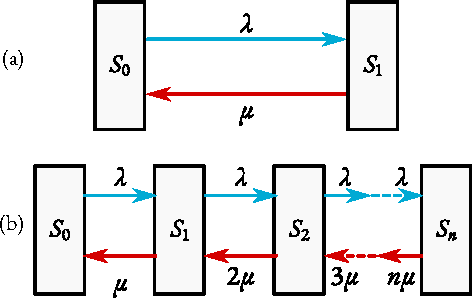
\includegraphics[width=0.75\tfwidth]{figures/state-graph3.pdf}
\caption{State graph of a system with losses.\label{state-graph3}}
 \end{figure}

We shall not go into detail on this type of system and go straight over
to a re general case, an \redem{n-server system with losses}. An example is
a system consisting of $n$ telephone lines. Erlang, the founder of the
queueing theory, considered precisely this system. The corresponding
state graph is given in \figr{state-graph3}~\drkgry{(b)}. The states of the system are designated as follows: $S_{0}$ when all servers are unoccupied, $S_{1}$ when one server is occupied and the others are unoccupied, $S_{2}$, when two servers are occupied while the others are unoccupied, and so on, and $S_{n}$ is the state
when all $n$ servers are occupied. As in the preceding example, $\lambda$ is the customer arrival rate, and $\mu$ is the service-completion rate.

Suppose the system is in state $S_{0}$. When a customer request arrives,
one of the servers becomes occupied, and the system is transferred to
state $S_{1}$. If the system is in state $S_{1}$, and a new customer arrives, two
servers become occupied, and the system is transferred from $S_{1}$ to $S_{2}$.
Thus, each customer (with the rate of arrivals $\lambda$) transfers the system
from one state to the adjacent one \redem{from left to right} (see the state graph
in the figure). The arrival of events leading to transitions to adjacent
states \redem{from right to left} is somewhat more complicated. If the system is
in the state $S_{1}$ (only one server is occupied), the next service-completion
event will disengage the server and transfer the system to state $S_{0}$. Let
me remind you that the service-completion rate is $\mu$. Now suppose the
system is in $S_{1}$, i.e. two servers are occupied. The average time of service
for each server is the same. Each sewer is disengaged with the rate
it when services are completed. As to the transition of the system from
$S_{2}$ to $S_{1}$, it is indifferent as to which of the two servers is unoccupied.
Therefore. events which transfer the system from $S_{2}$ to $S_{1}$ arrive at the
rate $2\mu$. As to the transition of the system from $S_{3}$ to $S_{2}$, it is indifferent as to which of the three occupied servers is disengaged. Events which
transfer the system from $S_{3}$ to $S_{2}$ arrive at the rate $3\mu$, and so forth. It is easy to see that the rate of event arrival which transfers the system from $S_{k}$ to $S_{k-1}$ is $k \mu$.

Let us assume that the system is in a steady state. Applying the rule
from the preceding section and using the state graph in \figr{state-graph3}~\drkgry{(b)}, we can compile the Chapman-Kolmogorov equations for the, probabilities $p_{0}, \, p_{1}, \, p_{2},\ldots{} p_{n}$, (recall that $p_{i}$ is the probability that the system is in the state $S_{i}$). We obtain the following system of equations:\\[-10pt]
\begin{equation}%
\left.
\begin{split}
\lambda p_{0} & = \mu p_{1},\\[-3pt]
(\lambda + \mu) p_{1} & = \lambda p_{0} + 2\mu p_{2},\\[-3pt]
(\lambda + 2 \mu) p_{2} & = \lambda p_{1} + 3\mu p_{3},\\[-3pt]
\ldots{} \quad \ldots{} \quad \ldots{} \quad \ldots{} , \\[-3pt]
(\lambda + k \mu) p_{k} & = \lambda p_{k-1} + (k+1)\mu p_{k+1},\\[-3pt]
\ldots{} \quad \ldots{} \quad \ldots{} \quad \ldots{} ,\\[-3pt]
[\lambda + (n-1) \mu] p_{n-1} & = \lambda p_{n-2} + n \mu p_{n},\\[-3pt]
p_{0} + p_{1} + p_{2} + \ldots{} + p_{n} & = 1.
\end{split}
\right\}
\label{eq-2.3}
%eq 2.3
\end{equation}
This set of equations can be solved easily, Using the first equation, we
can express $p_{1}$ in terms of $p_{0}$ and substitute it into the second equation. Then we can express $p_{2}$ in the second equation in terms of $p_{n}$ and substitute it into the third one, and so forth. At the last but one stage,
we express $p_{n}$ in terms of $p_{0}$. And finally, the results obtained at each
stage can be substituted into the last equation to find the expression for
$p_{0}$. Thus
\begin{equation}%
\begin{split}
p_{0} & =\left[ 1 + \frac{\lambda}{\mu} + \frac{(\lambda/\mu)^{2}}{2!}+ \frac{(\lambda/\mu)^{3}}{3!}+ \ldots + \frac{\frac{(\lambda/\mu)^{n}}{n!}}{} \right]^{-1},\\
p_{k} & = \frac{(\lambda/\mu)^{k}}{k!} p_{0} \,\, (k= 1,\, 2, \, 3 \, n).
\end{split}
\label{eq-2.4}
\end{equation}
A customer’s request is refused if it arrives when all $n$ servers are engaged, i.e. when the system is in state $S_{n}$. The probability that the system
is in $S_{n}$ equals $p_{n}$, This is the probability that a customer arriving at the system is refused and the service‘is not rendered. We can find the
probability that a customer arriving at the system will he served,
\begin{equation}%
Q = 1 - p_{n} = 1 - \frac{(\lambda/\mu)^{n}}{n!}\, p_{0}.
\label{eq-2.5}
%eq(2.5)
\end{equation}
By multiplying $Q$ by $\lambda$, we obtain the service-completion rate of the
system. Each occupied server serves $\mu$ customers per unit time, so we
can divide $Q$ by $\mu$ and find the average number of occupied servers in
the system,
\begin{equation}%
E(N) = \frac{\lambda}{\mu} \left( 1 - \frac{(\lambda/\mu)^{n}}{n!}  p_{0} \right).
\label{eq-2.6}
%eq(2.6)
\end{equation}

\txthead{How many servers are required?} Let us consider a concrete example.
Suppose a telephone exchange receives 1.5 requests per minute on the
average, and the service completion rate is 0.5 request per minute (the average service time for one customer is two minutes). Therefore, $\lambda/\mu = 3$. Suppose the exchange has three servers (three telephone lines). Using formulas \eqref{eq-2.4}--\eqref{eq-2.6} for $\lambda/\mu = 3$ and $n = 3$, we can calculate that the probability of servicing the arriving customers is only 65 per cent. The average number of engaged lines is 1.96, which is 65 per cent of the total number of lines. Thus, 35 per cent of the customers are refused and not served. This is too much. 

We may decide on increasing the number of servers. Suppose we add one more, a fourth line. Now the probability of a customer being served increases to 79 per cent (the probability of being turned away decreases to 21 per cent). The average number of engaged lines becomes 2.38, which is 60 per cent of the total number of lines. It would appear that the decision to install a fourth line is reasonable because a relatively small reduction in the percentage of occupied servers (from 65 to 60 per cent) results in a significant rise in the probability to be served, from 65 to 79 per cent. Any further increase in the number of lines may become unprofitable because the effectiveness of the system may fall due to the increasing idleness of the lines. A more detailed analysis would then be required to allow for the cost of installing each new line. Let me remark that at $n = 5$ we get $Q= 89$ per cent and $E(N)/n = 53$ per cent, while for $n= 6, \, Q= 94$ per cent and $E (N)/n = 47$ per cent.

\txthead{Single-server systems with finite queues.} Suppose	the	number of queueing customers is restricted, and the queue may only accommodate $m$ customers. If all places in the queue are occupied, a newcomer is turned away. For example, a petrol station with only one pump (only one server) and a parking area for no more than $m$ cars. If all the places at the station are occupied, the next car arriving at the station will not stop and will go on to the next.
 \begin{figure}[!h]
 \centering
 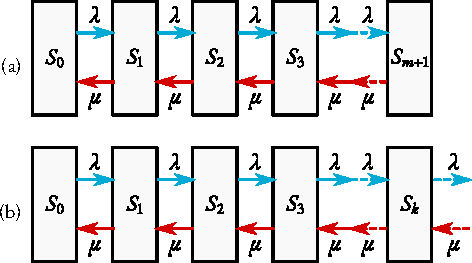
\includegraphics[width=0.75\tfwidth]{figures/state-graph4.pdf}
\caption{State graph for a system (a) with finite queues and (b) with infinite queues.\label{state-graph4}}
%fig 2.4
 \end{figure}
The state graph for this system is shown in \figr{state-graph4}~\drkgry{(a)}. Here $S_{0}$ means the server is unoccupied, $S_{1}$  the server is occupied, $S_{2}$  the server is occupied and there is one customer in the queue, $S_{3}$ the server is occupied and there are two customers in the queue, $\ldots{}, S_{m+1}$ means the server is occupied and there are $m$ customers in the queue. As before, $\lambda$ is the customer arrival rate and $\mu$ is the service completion rate. The Chapman-Kolmogorov equations for steady state are
\begin{equation}%
\left.
\begin{split}
\lambda p_{0} & = \mu p_{1},\\
(\lambda + \mu) p_{1} & = \lambda p_{0} + 2\mu p_{2},\\
\ldots{} \quad \ldots{} \quad & \ldots{} \quad \ldots{} , \\
(\lambda + \mu) p_{m} & = \lambda p_{m-1} + \mu p_{m+1},\\
p_{0} + p_{1} + p_{2} + \ldots + p_{m} + p_{m+1} & = 1.
\end{split}
\right\}
\label{eq-2.7}
%eq 2.7
\end{equation}
By solving this system and introducing the designation $\rho = \lambda/\mu$ we obtain
\begin{equation}%
p_{0} = \frac{1}{1 + \rho+ \rho^{2}+ \rho^{3}+ \ldots + \rho^{m+1}} = \frac{1 - \rho}{1 - \rho^{m+2}}, \quad  p_{k}= \rho^{k} p_{0}.
\label{eq-2.8}
%eq2.8
\end{equation}
A customer is turned away if the server is engaged and there are $m$ customers in the queue, i.e. when the system is in the state $S_{m+1}$. Therefore, the probability a customer is turned away is $p_{m+1}$. The average number of customers in the queue is evidently
\begin{equation*}%
E(r) = \sum_{k=1}^{m} k p_{k+1}
\end{equation*}
($p_{k+1}$ is the probability of $k$ customers being in the queue). The average
waiting time in the queue is the ratio $E (r)/\lambda$.

Suppose one car arrives at the petrol station per minute ($\lambda = 1$
customer per minute) and a car is filled, on average, within two minutes
$(\mu= 1/2)$. Therefore, $p = \lambda/\mu = 2$. If the number of places in the queue $m = 3$, it is easy to calculate that the probability of a customer being
refused is 51.6 per cent while the average waiting time in the queue is
2.1 min. Suppose that in order to decrease the probability of a customer
being refused we double the number of places in the queue. It turns out
that at $m = 6$ the probability of refusal is 50.2 per cent, i. e. it is, in fact, the same, but the waiting time in the queue noticeably increases to
5 min. It is clear from \eqref{eq-2.8} that if $\rho > 1$, the probability of being refused stabilizes with increasing $m$ and tends, to $(\rho - 1)/\rho$. In order to reduce the probability of being refused significantly, it is necessary (if it is not possible to decrease $\rho$) to use multi-server systems.

\txthead{Single-server systems with infinite queues.} This sort of queueing
system is rather common: for example, a doctor receiving patients,
a single public telephone, or a port with only one berth at which
a single ship can unload. The state graph for the system is given in
\figr{state-graph4}~\drkgry{(b)}. Here So means that the server is unoccupied, $S_{1}$ the server is occupied, $S_{2}$ the server is occupied and there is one customer in the queue, $S_{3}$ the server is occupied and there are two customers in the queue, and $S_{k}$ means that the server is occupied and there are $k - 1$
customers in the queue, and so on.

Up till now, we considered graphs with a finite number of states. However, here is a system with an infinite number of discrete states. Is it possible to discuss a steady state for such a system? In fact we can. It is only necessary that the inequality $\rho < 1$ holds true. If so, then the sum
$1 + \rho+ \rho^{2}+ \rho^{3}+ \ldots{} + \rho^{m+1}$ in \eqref{eq-2.8} can be substituted by the sum of the decreasing geometric progression $1 + \rho+ \rho^{2}+ \rho^{3}+ \ldots{}  = 1/(1 - \rho)$. The result is
\begin{equation}%
p_{0} = 1 - \rho  \qand  p_{k} = \rho^{k} p_{0}.
\label{eq-2.9}
\end{equation}
If $\rho \geqslant 1$, then the system does not have a steady state, i.e. the queue increases infinitely as $t \to \infty$.

\section{Method of Statistical Testing}

A \redem{statistical testing} involves numerous repetitions of uniform trials. The
result of any individual trial is random and is not of much interest.
However, a large number of results is very useful. It shows some
stability (\redem{statistical stability}) and so the phenomenon being investigated
in the trials can be described quantitatively. Let us consider a special
method for investigating a random process based on statistical testing.
The technique is commonly called the \redem{Monte Carlo method}.

In fact neither the city of Monte Carlo, the capital of the independent
principality of Monaco nor its inhabitants nor guests are in any way
related to the considered method. Instead, the city is known for its
casinos where tourists pay good money playing roulette, and a roulette
wheel could be the city's emblem. At the same time, a roulette is
a generator of random numbers and this is what is involved when the
Monte Carlo method is used.

\txthead{Two examples indicating the usefulness of statistical testing.} 

\redem{First example.} Look at \figr{monte-carlo1}. It contains a square with side $r$ in which a quarter circle of radius $r$ is inscribed. The ratio of the yellow area to the area of the square is $(\pi r^{2})/4r^{2} = \pi /4$. This ratio and, therefore, the value of $n$ can be obtained using the following statistical test. Let us place a sheet of paper with the figure on a horizontal surface and let us throw small grains on this paper. We should not aim so that any grain
can fall on any part of the paper with equal probability. It is possible,
for instance, to blindfold the person throwing the grains. The grains will
be distributed over the surface of the paper in a random fashion
(\figr{monte-carlo1}~\drkgry{(b)}). Some will land outside the square, but we shall not consider them. We now count the number of grains within the square (and call
this number $N_{1}$) and count the grains within the yellow area (calling it
$N_{2}$). Since any grain may land with equal probability on any part of the
figure, the ratio $N_{2}/N_{1}$ when the number of trials is large, will
approximate the ratio of the yellow area to the area of the square, i.e.
the number $\pi /4$. This approximation will become more accurate as the
number of trials increases.
 \begin{figure}[!h]
 \centering
 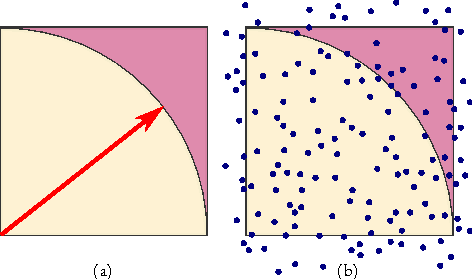
\includegraphics[width=0.85\tfwidth]{figures/monte-carlo1.pdf}
\caption{Finding out value of $\pi$ using a random distribution.\label{monte-carlo1}}
%fig 2.6
 \end{figure}
This example is interesting because a definite number (the number $\pi$)
can be found following a statistical testing. It can be said that
randomness is used here to obtain a deterministic result, an
approximation of the real number $\pi$.


\redem{Second example}. Statistical testing is used much more commonly to
investigate \redem{random events} and \redem{random processes}. Suppose someone
assembles a device consisting of three parts ($A$, $B$, and $C$). The assembler
has three boxes containing parts $A$, $B$, and $C$, respectively. Suppose half
the parts of each type are larger than the standard and the other half
are smaller. The device cannot operate when all three parts are larger
than the norm. The assembler takes the parts from the boxes at random.
What is the probability that a normally operating device will be
assembled?

Naturally, this example is rather simple and the probability can easily
be calculated. The probability of assembling a device that does not work
is the probability that all three parts will be larger than the norm, and
this equals $1/2 \times 1/2 \times 1/2 = 1/8$. Therefore, the probability that
a normally operating device will be assembled is $1 - 1/8 = 0.875$.

Let us forget for a time that we can calculate the probability and
instead use statistical testing. We should choose trials such that each
one has equally probable outcomes, for instance, tossing a coin. Let us
take three coins: $A$, $B$, and $C$. Each coin corresponds to a part used to
assemble the device. Heads will mean that the respective part is larger
than the norm while tails will mean that it is smaller. Having agreed on
this, let us start the statistical testing. Each trial involves tossing all
three coins. Suppose after $N$ trials ($N \gg 1$) three heads were recorded in
$n$ trials. It is easy to see that the ratio $(N - n)/N$ is the approximation of
the probability in question.

Naturally, we could use any other random number generator instead
of coins. It would also be possible, for instance, to throw three dice,
having agreed to relate three faces of each die with larger than normal
parts and three faces with smaller parts.

Let me emphasize that the randomness in these examples was
a positive factor rather than a negative one, and was a tool which
allowed us to obtain a needed quantity. Here chance works for us rather
than against us.

\txthead{Random number tables come into play.} Nobody uses statistical
testing in simple practical situations like the ones described above. It is
used when it is difficult or even impossible to calculate the probability
in question. Naturally you might ask whether a statistical testing would
be too complicated and cumbersome. We threw grains or three coins in
the examples. What will be required in complicated situations? Maybe,
there will be practically unsurmountable obstacles?

In reality, it is not necessary to stage a statistical experiment with
random trials. Instead of real trials (throwing grains, dice, etc.), we need
only use \redem{random number tables}. Let me show how this can be done in
the above two examples.
 \begin{figure}[!h]
 \centering
 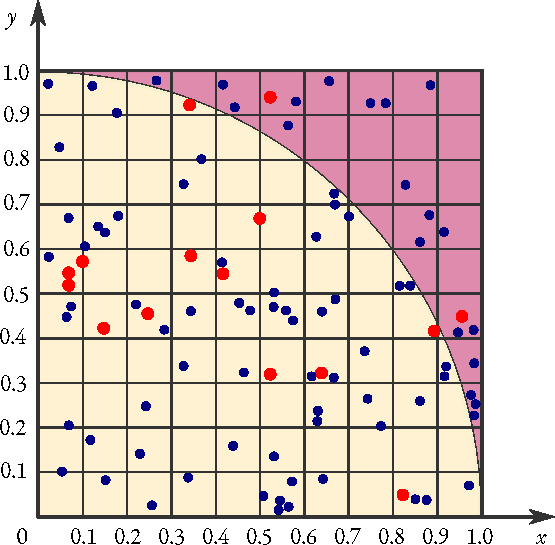
\includegraphics[width=0.75\textwidth]{figures/monte-carlo2.pdf}
\caption{Finding out value of $\pi$ using a random number table.\label{monte-carlo2}}
%fig 2.7
 \end{figure}
 
\redem{First example.} Let us again discuss the picture in \figr{monte-carlo1}. We now plot two coordinate axes along the sides of the square and select the scales such that the side of the square equals unity (\figr{monte-carlo2}). Now instead of throwing grains, we take the random number table in \figr{random-table} and divide each number by \num{10000} so that we obtain a set of random numbers between 0 and 1. We take the numbers in the odd lines as $x$-coordinates and the ones directly below as the $y$-coordinates of random points. We plot the points onto the diagram, systematically
moving along the random number table (for instance, first down the first
column from top to bottom, and then down the second column, and so
on). The first fifteen random points are shown in the picture in red, and
they have the coordinates as shown in \tabl{random-coord}.%\\[-15pt]
\begin{wrapfloat}{table}{O}{\mfwidth}
\centering
\begin{smaller}
\begin{tabular}{l}
(0.0655, 0.5255) \\
 (0.6314, 0.3157) \\
  (0.9052, 0.4105) \\
(0.1437, 0.4064) \\
 (0.1037, 0.5718) \\
  (0.5127, 0.9401) \\
(0.4064, 0.5458) \\ 
(0.2461, 0.4320) \\ 
(0.3466, 0.9313) \\ 
(0.5179, 0.3010) \\ 
(0.9599, 0.4242) \\
 (0.3585, 0.5950) \\ 
(0.8462, 0.0456) \\
 (0.0672, 0.5163) \\
  (0.4995, 0.6751) \\
\end{tabular}
\end{smaller}
%\end{center}
\caption{Coordinates of fifteen random numbers shown in red in the \figr{monte-carlo2}. \label{random-coord}}
\end{wrapfloat}
The figure contains 85 random points in black. From
the diagram, it is easy to calculate that using the first fifteen points
$N_{2}/N_{1}= 13/15$ and therefore $\pi = 3.47$ while for a hundred points
$N_{2}/N_{1}= 78/100$ and therefore $\pi = 3.12$.

\redem{Second example.} Instead of tossing coins, we can use the same random
number table (see \figr{random-table}). Each number over \num{5000} can be replaced by a ``+'' sign and the rest replaced by a ``$-$'' sign. The result is a table
consisting of a random set of pluses and minuses. We divide these signs
into triples as shown in \figr{monte-carlo3}. Each triple corresponds to a set of three parts. A ``+'' sign means that a part is larger than the norm while
a ``$-$'' sign means it is smaller. The approximation of the sought
probability is the ratio $(N - n)/N$, where $N$ is the total number of triples
and $n$ is the number of triples with three pluses (they are shaded in the
figure). It can be seen that $(N - n)/N = 0.9$ in this case, and this is close
enough to the accurate value 0.875.
 \begin{figure}[!h]
 \centering
 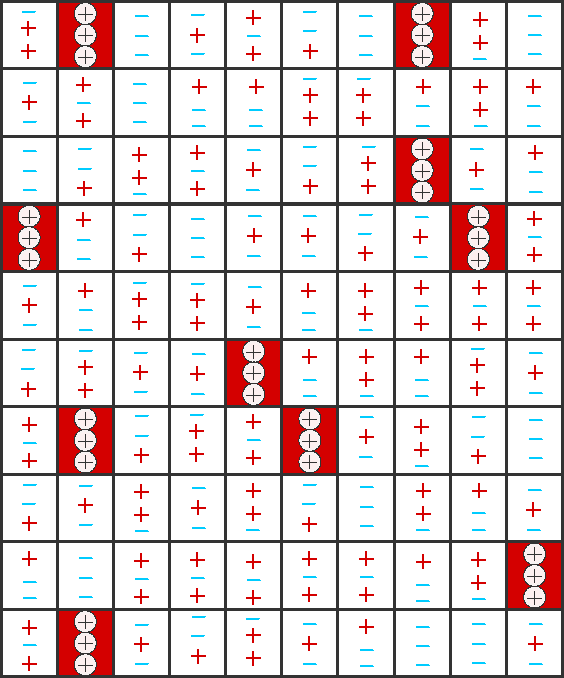
\includegraphics[width=0.75\tfwidth]{figures/monte-carlo3.pdf}
\caption{Using a random number table instead of coin tosses for statistical testing.\label{monte-carlo3}}
%fig 2.7
 \end{figure}

Thus, we have reduced statistical testing to operations on a random
number table and used our desk instead of an experimental bench.
Rather than performing very many trials, we just look at a random
number table.

\txthead{Computers come into play.} Instead of sweating over a random
number table, we could program a computer to do the job. We place
a random number table in the computer's memory and program it to
search the random numbers and sort them as necessary. In our two
examples, we would do the following.

\redem{First example}. The computer has to check the coordinates of each
random point to see whether $x^{2} + y^{2} < 1$. It counts the number of points
for which this is true (the number is $N_{2}$) and the number of points for
which it is false (this number of points will be the difference $N_{1} - N_{2}$).

\redem{Second example}. All random numbers in the computer's memory must
be divided into triples and the triples checked to find ones in which all three numbers are over 5000. The number of such triples is $n$.

\txthead{The Monte Carlo method.} The world changed when the computer
came into play. By processing a random number table the computer
simulates the statistical testing and it can do this many times faster than
could be done either experimentally or by working manually with
a random number table. And now we come to the Monte Carlo method,
a very useful and efficient method of probabilistic calculation which is
applied to many problems, primarily those that cannot be solved
analytically.

Let me emphasize two points. \redem{Firstly}, the Monte Carlo method
utilizes \redem{randomness not chance}. We do not try to analyze the complicated random processes, nor even simulate them. Instead, we use randomness, as it were, to deal with the complications chance has engendered.

Chance complicates our investigation and so randomness is used to
investigate it. \redem{Secondly}, this method is \redem{universal} because it is not restricted by any assumption, simplification, or model. There are two
basic applications. The first is the investigation of random processes
which cannot be dealt with analytically due to their complexity. The
second is to verify the correctness and accuracy of an analytical model
applied in concrete situations.

The Monte Carlo method was first widely used in operations research,
in looking for optimal decisions under conditions of uncertainty, and in
treating complicated multi-criterial problems. The method is also successfully
used in modern physics to investigate complex processes involving
many random events.

\txthead{A Monte Carlo simulation of a physical process.} Let us consider the
flow of neutrons through the containment shield of a nuclear reactor.
Uranium nuclei split in the core of the reactor and this is accompanied
by the creation of high-energy neutrons (of the order of several million
electron volts). The reactor is surrounded by a shield to protect the
working areas (and therefore, the personnel) from the radiation. The
wall is bombarded by an intense flow of neutrons from the reactor core.
The neutrons penetrate into the wall and collide with the nuclei of the
atoms of the wall. The result is that the neutrons may either be
absorbed or scattered. If scattered, they give up some of their energy to
the scattering nuclei.

This is a complicated physical process \redem{involving many random events}.
The energy and the direction of a neutron when it leaves the reactor
core and enters the wall are random, the length of the neutron path
before it first collides is random, the nature of collision (absorption or
scattering) is random, the energy and the direction of the scattered
neutron are random, etc. Let me show in general how the Monte Carlo
method is applied to analyze the process. Obviously the computer is
first programmed with data on the elementary collisions between
neutrons and the wall nuclei (the probabilities of absorption and
scattering) the parameters of the neutron flow into the wall, and the
properties of the wall. The computer model simulates a neutron with
a randomly selected energy and direction (when it leaves the reactor
core and enters the wall) in line with appropriate probabilities. Then it
simulates (bearing in mind the relevant probabilities) the flight of the
neutron until it first collides. Then the first collision is simulated. If the
neutron is not absorbed, subsequent events are simulated, i.e. the
neutron's flight until its second collision, the collision itself, and so on.
The ``history'' of the neutron is determined from the moment it
penetrates the wall until it is either absorbed, scattered back into the
reactor core, or scattered into the working area. 

The computer simulation is repeated for very many neutrons until a set of possible
trajectories of neutrons within the wall is obtained (\figr{neutron-path}). Each trajectory is the result of one statistical trial simulating the ``history'' of
Chance complicates our investigation and so randomness is used to
investigate it. Secondly, this method is universal because it is not
restricted by any assumption, simplification, or model. There are two
an individual neutron. Given an enormous set of trials the neutron flow
through the containment wall as a whole can be analyzed and
recommendations for the thickness of the wall and its composition can
be made so as to guarantee the safety of the personnel working at the
reactor.
 \begin{figure}[!h]
 \centering
 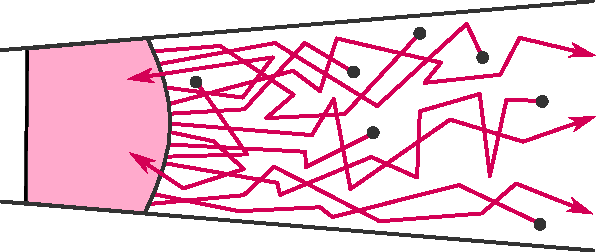
\includegraphics[width=0.85\tfwidth]{figures/neutron-path.pdf}
\caption{A set of all possible trajectories for the neutron.\label{neutron-path}}
%fig 2.9
 \end{figure}

Modern physics requires the Monte Carlo method on many
occasions. Physicists use it to investigate cosmic-ray showers in the
Earth's atmosphere, the behaviour of large flows of electrons in electron
discharge devices, and the progress of various chain reactions.

\section{Games and Decision Making}

\txthead{What is the theory of games?} Suppose we must make a decision when
our objectives are opposed by another party, when our will is in conflict
with another will. Such situations are common, and they are called
\redem{conflict situations}. They are typical for military actions, games, and
every-day life. They often arise in economics and politics.

A hockey player makes a decision that takes into account the current
situation and the possible actions of the other players. Every time
a chess player makes a decision, he (or she) has to consider the
counteraction of the opponent. A military decision should allow for the
retaliation of the enemy. In order to decide at what price to sell
a product, a salesman must think over the responses of the buyer. In
any election campaign, each political party in a capitalist country tries
to foresee the actions of the other parties that are competing for power.
In each case, there is a collision of opposing interests, and the decision
must be related with \redem{overcoming a conflict}.

Decision making in a conflict situation is hampered by \redem{uncertainty
about the behaviour of the opponent}. We know that the opponent will try
to act in a way that is least advantageous for us in order to ensure the
greatest advantage for himself. However, we do not know to what extent
our opponent is able to evaluate the situation and the possible
consequences and, in particular, how he evaluates our options and
intentions. We cannot predict the actions of the opponent accurately,
and the opponent cannot predict our actions. But nonetheless, we both
have to make decisions.

Because some way of justifying an \redem{optimal} decision was needed in
conflict situations, a new mathematical discipline arose, the \redem{theory of
games}. The ``game'' here is a mathematical model of a conflict situation.
Unlike a real conflict, a game has definite rules which clearly indicate
the rights and duties of the participants and the possible outcomes of
the game (a gain or loss for each participant). Long before the
emergence of game theory, simple models of conflicts were used widely.
I mean games in the literal sense of the word: chess, checkers or
draughts, dominoes, card games, etc. In fact, the name of the theory and
the various terms used in it are all derived from these simple models.
For instance, the conflicting parties are called players, a realization of
a game is a match, the selection of an action by a player (within the
rules) is a move.

There are two kinds of move, personal and chance ones. A \redem{personal}
move is when the player conscientiously selects an action according to
the rules of the game. A \redem{chance} move does not depend on the player's
will: it may be determined by tossing a coin, throwing a die, taking
a card from a pack, etc. Games consisting of only chance moves are
called \redem{games of chance}, or \redem{games of hazard}. Typical examples are lotteries and bingo. Games with personal moves are called \redem{strategic}.
There are strategic games consisting exclusively of personal moves, for
instance, chess. There are also strategic games consisting of both
personal and chance moves, for instance, certain card games. Let me
remark that the uncertainty in games with both personal and chance
moves involve both sorts of randomness: the uncertainty of the result of
the chance moves and the uncertainty of the opponent's behaviour in his
personal moves.

Game theory is not interested in gambles. It only deals with strategic
games. The aim of the game theory is to determine the player's strategy
so as to maximize his chances of winning. The following basic
assumption underlies the search for optimal strategies. It is assumed that
the opponent is as active and as reasonable as the player, and he or she
also takes attempts to succeed.

Naturally, this is not always true. Very often our actions in real
conflicts are not as good as they could be when we assume reasonable
behaviour from our adversary; it is often better to guess at the ``soft
spots'' of the opponent and utilize them. Of course, we take a risk when
doing so. It is risky to rely too much on the soft spots of the opponent,
and game theory does not consider risk. It only detects the most
cautious, ``safe'' versions of behaviour in a given situation. It can be said
that game theory gives wise advice. By taking this advice when we make
a practical decision, we often take a conscientious risk. E. S. Wentzel
writes in \redem{Operations Research}: 
\begin{quote}
``Game theory is primarily valuable in
terms of the formulation of the problem, which teaches us never to forget that the opponent also thinks and to take into account his possible tricks and traps. The recommendations following from the
game approach are not always concrete or realizable, but it is still
useful, while taking a decision, to utilize a game model as one of several
possible ones. But the conclusions proceeding from this model should
not be regarded as final and indisputable.''
\end{quote}

\txthead{The payoff matrix of a game} \redem{Finite two-person zero-sum games} are the best investigated types in game theory. A \redem{two-person} game is a game in which there are exactly two players or conflicting interests. A game is \redem{finite} if both players have a finite number of possible strategies, i.e. a finite number of behaviours. When making a personal move, a player
follows a strategy. A \redem{zero-sum} game is a game where the gain by one
player equals the loss by the other.

 \begin{figure}[!h]
 \centering
 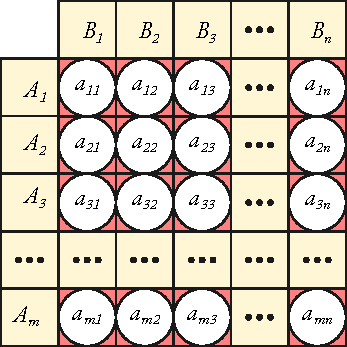
\includegraphics[width=0.6\tfwidth]{figures/two-player1.pdf}
\caption{Strategies in a finite two-person zero-sum game.\label{twoplayer1}}
%fig 2.10
 \end{figure}

Suppose there is a finite two-person zero-sum game where player
$A$ has $m$ strategies and player $B$ has $n$ strategies (an $m \times n$ game). We use $A_{1}, \, A_{2}, \ldots, A_{m}$ to denote the strategies available to player $A$ and $B_{1}, \, B_{2}, \ldots, B_{n}$ the strategies available to player $B$. Suppose player $A$ makes a personal move and selects a strategy $A_{i} (1 \leqslant i \leqslant m)$, and player $B$ at the same time selects strategy $B_{j} (1 \leqslant j \leqslant n)$. We use $a_{ij}$ to denote the gain of player $A$. Let us identify ourselves with player $A$ and consider each move from his viewpoint. The gain $a_{ij}$ may be either a real gain or a loss (a loss would be a negative gain). The set of gains $a_{ij}$ for different values of $i$ and $j$ can be arranged in matrix form with the rows corresponding to player $A$ strategies and the columns to player $B$ strategies (\figr{twoplayer1}). This is called the \redem{payoff matrix} for the game.

Consider the following game. Each player, $A$ and $B$, writes, simultaneously
and independently, one of three numbers 1, 2, or 3. If the sum of
the numbers is \redem{even}, player $B$ pays player $A$ the sum, while if the sum is \redem{odd}, $A$ pays it to $B$. Player $A$ has three strategies: $A_{1}$ to write 1, $A_{2}$ to write 2, and $A_{3}$ to write 3. Player $B$ has the same strategies. The game is a $3 \times 3$ one because its payoff matrix contains three rows and three columns. This matrix is given in Figure \ref{twoplayer2}(a). Note that a gain by player $A$ of, for instance, $-3$ is a loss in reality because $A$ pays 3 units to $B$. 

 \begin{figure}[!h]
 \centering
 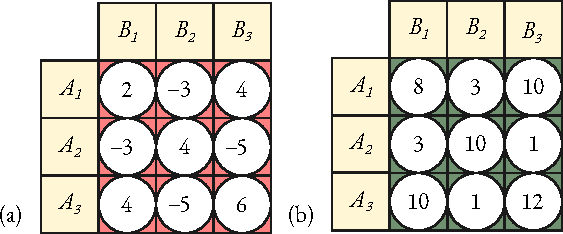
\includegraphics[width=0.85\tfwidth]{figures/two-player2.pdf}
\caption{A payoff matrix in a $3 \times 3$ finite two-person zero-sum game.\label{twoplayer2}}
%fig 2.11
 \end{figure}


Some of the elements are positive and the others are negative in the matrix in Figure \ref{twoplayer2}(a). It is possible to make all the elements of the payoff matrix positive by adding some number, say 6, to each element of the
matrix. We obtain the matrix in Figure \ref{twoplayer2}(b). This matrix is equivalent to the initial one from the viewpoint of analyzing optimal strategies.

\txthead{The minimax principle} Let us analyze the game using. the payoff
matrix in \figr{twoplayer2}(b). Suppose we (player $A$) pick strategy $A_{i}$. Then, depending on the strategy selected by player $B$, our gain may be either 8 or 3 or 10. Thus, strategy $A_{1}$ yields a gain of 3 in the worst case. If we choose either $A_{2}$ or $A_{3}$, the worst gain is 1. Let us write down the
minimum possible gains for each strategy $A_{i}$ as an additional column in
the payoff matrix (\figr{twoplayer3}). It is clear that we should choose a strategy whose \redem{minimum possible gain is greatest} (as compared with the other strategies). This is strategy $A_{1}$ in this case. Three is the largest one out of the minimum gains for each strategy (viz. 3, 1, and 1). This is called
the \redem{maximin gain}, or the \redem{maximin}, or just the \redem{maxim}. It is also sometimes called the \redem{lower value of the gain}. Thus, if we select the maximin strategy (strategy $A_{1}$ in this case), our gain is guaranteed to be, whatever the behaviour of the opponent, at least the lower value of the game (a gain of 3 in this case). The opponent will reason in a similar way. If he selects
strategy $B_{1}$, he will have to give us a gain of 10, which is his worst case.

 \begin{wrapfigure}{O}{\mfwidth}
 \centering
 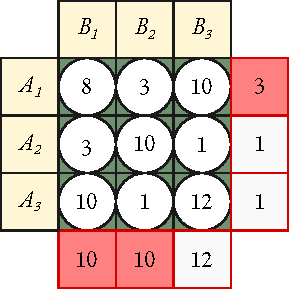
\includegraphics[width=0.9\linewidth]{figures/two-player3.pdf}
\caption{A payoff matrix in a $3 \times 3$ finite two-person zero-sum game.\label{twoplayer3}}
%fig 2.12
 \end{wrapfigure}
The same can be said of strategy $B_{2}$. Strategy $B_{3}$ yields the worst case
for the opponent corresponding to a gain of 12 for us. Numbers 10, 10,
and 12 are the maximum values of our gains corresponding to the
opponent's strategies $B_{1}$, $B_{2}$, and $B_{3}$, respectively. Let us write these values as a row in the payoff matrix (see \figr{twoplayer3}). It is clear that our opponent should select the strategy which \redem{minimizes} our \redem{maximum possible gain}. This is either strategy $B_{1}$ or $B_{2}$. Both strategies are minimax ones and both guarantee that our opponent limits our gain to the \redem{minimax}, or, in other words, the \redem{upper value of the game} is 10.

Our maximin strategy and the minimax strategy of the opponent are
the most cautious ``safe'' strategies. The principle of being cautious
dictating that the players select such strategies is called the \redem{minimax
principle}.

Now let us return to the matrix in \figr{twoplayer3} and try some reasoning. The opponent has two minimax strategies,  $B_{1}$ and  $B_{2}$. Which strategy should he choose? If he knows that we are cautious and have selected the maximin strategy  $A_{1}$ he would not select strategy  $B_{1}$ because this would yield a gain of 8. Therefore, it is likely that he would choose
strategy $B_{2}$, and our gain would then be 3. But if we perceived our
opponent's ideas correctly, shouldn't we take a risk and choose strategy
 $A_{2}$? If the opponent then selects strategy  $B_{2}$, our strategy  $A_{2}$ will give us a gain of 10. However, our deviation from the minimax principle may
cost us dearly. If the opponent is even cleverer and reasons in a similar
way, he would answer our strategy  $A_{2}$ with strategy  $B_{3}$ rather than  $B_{2}$. And then, instead of a gain of 10, we would only gain 1.

Does this mean that game theory only recommends we adhere to
a minimax (maximin) strategy? It depends on whether the payoff matrix
has a \redem{saddle point}.

\txthead{A game with a saddle point.} Consider the $3 \times 3$ game, whose payoff matrix is given in \figr{saddle-point}. Here both the maximin and minimax gain 4. In other words, the lower and the upper value of the game coincide and both are equal to 4. A gain of 4 is simultaneously the maximum of
the minimum gains for strategies $A_{1}, \, A_{2}$, and $A_{3}$ and the minimum of the maximum gains for strategies $B_{1}, \, B_{2}$, and $B_{3}$. In geometry, the point on a surface which is at the same time a minimum along one coordinate axis and a maximum along the other is called a saddle point. Point $C$ on the surface in \figr{saddle-point} is a \redem{saddle point}. It is the maximum along the $x$-axis and the minimum along the $y$-axis. It is easy to see that the surface in the vicinity of this point is actually like a saddle. Just as in geometry, element $a_{22} = 4$ of the payoff matrix in question is called the
\redem{saddle point of the matrix}, and the game is said to have a saddle point.

 \begin{figure}[!h]
 \centering
 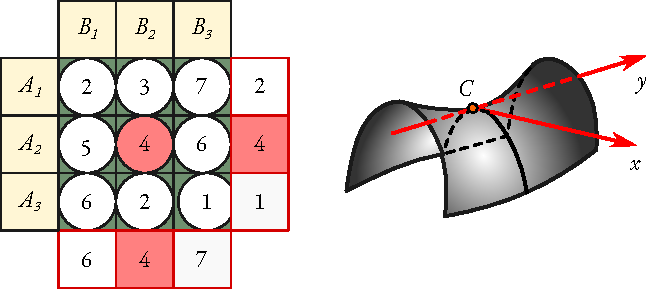
\includegraphics[width=\tfwidth]{figures/saddle-point.pdf}
\caption{A $3 \times 3$ game with saddle point.\label{saddle-point}}
%fig 2.13
 \end{figure}
We need only look through the matrix in \figr{saddle-point}, to see that each player should adhere to his maximin (minimax) strategy. These strategies
are optimal in a game with a saddle point. Any deviation from them will
be disadvantageous for the player who took the risk.

However, if a game does not have a saddle point (see the matrix in
\figr{twoplayer2}), neither of strategies $A_{i}$ or $B_{j}$ is optimal.

\txthead{The necessity of a random change of strategy in a game without
a saddle point.} Suppose that we and our opponent repeatedly play the
game whose matrix is given in \figr{twoplayer2}. If we choose a definite strategy, for instance, the maximin strategy $A_{1}$, and adhere to it turn after turn, our opponent will see it and select strategy $B_{2}$ each time, so that our
gain will not exceed the lower value of the game, i.e. it will equal 3.
However, if we suddenly (for the opponent) choose strategy $A_{2}$ instead
of $A_{1}$, we receive a gain of 10. Having guessed our new strategy
(naturally, if we later adhere to it), our opponent will go from strategy
$B_{2}$ to strategy $B_{3}$ right away, thus decreasing our gain to 1. And so
forth. We can see here a general rule for games without a saddle point:
a player using a \redem{certain strategy} will be worse off than a player who
\redem{changes strategy at random}.

However, the random changes in strategies should be done wisely
rather than haphazardly. Suppose $A_{1}, \, A_{2}, \ldots, A_{m}$ are the possible
strategies of player $A$ (see \figr{twoplayer1}). To obtain the greatest benefit, the strategies should be chosen at random but with different (specially
calculated) probabilities. Suppose strategy $A_{1}$ is used with probability
$p_{1}$, strategy $A_{2}$ with probability $p_{2}$ etc. Player $A$ is now said to have a \redem{mixed strategy} $S_{A} (p_{1}, \, p_{2}, \ldots{}, p_{m})$. Unlike $S_{A}$, the $A_{j}$ strategies are called \redem{pure strategies}. By correctly selecting the probabilities $p_{j}$ a mixed strategy may be \redem{optimal}. The gain of player $A$ will then be no less than a certain value $\nu$ called the \redem{value of the game}. This value is greater than the lower value of the game, but less than the upper one.

Player $B$ should behave in a similar manner. His optimal strategy is
also a mixed strategy. Let us designate it  $S_{B} (q_{1}, \, q_{2}, \ldots{}, q_{n})$, where $q_{j}$ are specially selected probabilities with which player $B$ uses strategies $B_{j}$. When player $B$ selects an optimal mixed strategy, the gain of player $A$ will be no more than game value $\nu$.

\txthead{The search for an optimal mixed strategy.} Let us use $S_{A} (p_{1}, \, p_{2}, \ldots{}, p_{m})$ to denote an optimal mixed strategy for player $A$. We must now find probabilities $p_{1}, \, p_{2}, \ldots{}, p_{m}$ and calculate the game value $\nu$ once the payoff matrix of the game is known (see \figr{twoplayer1}). Suppose player $B$ selects pure strategy $B_{1}$. Then the average gain of player $A$ will be $a_{11}p_{1} + a_{21}p_{2}+ \ldots{} + a_{m1}p_{m}$ This gain should be no less than the game value $\nu$, and hence
\begin{equation*}%
a_{11}p_{1} + a_{21}p_{2}+ \ldots + a_{m1}p_{m} \geqslant \nu.
\end{equation*}
If player $B$ selects strategy $B_{2}$, the average gain of player $A$ should also
be no less than the game value $\nu$, and hence
\begin{equation*}%
a_{12}p_{1} + a_{22}p_{2}+ \ldots + a_{m2}p_{m} \geqslant \nu.
%\label{b-strategy2}
% eq-2.10
\end{equation*}
Whichever strategy player $B$ chooses, the gain of player $A$ should
always be no less than the game value $\nu$. Therefore, we can write the
following system of $n$ inequalities (recall that $n$ is the number of $B$'s pure
strategies):
\begin{equation}%
\left.
\begin{split}
a_{11}p_{1} + a_{21}p_{2}+ \ldots + a_{m1}p_{m} & \geqslant \nu, \\
a_{12}p_{1} + a_{22}p_{2}+ \ldots + a_{m2}p_{m} & \geqslant \nu, \\
\ldots \quad \ldots \quad \ldots  \quad \ldots, \\
a_{1n}p_{1} + a_{2n}p_{2}+ \ldots + a_{mn}p_{m} & \geqslant \nu. \\
\end{split}
\right\}
\label{eq-2.10}
%eq-2.10
\end{equation}
Recall that
\begin{equation}
p_{1} + p_{2}+ \ldots + p_{m} = 1.
\label{eq-2.11}
%eq 2.11
\end{equation}
Introducing designations $x_{1} = 	p_{1}/\nu, \, x_{2} = p_{2}/\nu, \ldots x_{m} = 	p_{m}/\nu$ we can rewrite \eqref{eq-2.10} and \eqref{eq-2.11} as
\begin{equation}%
\left.
\begin{split}
a_{11}x_{1} + a_{21}x_{2}+ \ldots + x_{m1}p_{m} & \geqslant 1, \\
a_{12}x_{1} + a_{22}x_{2}+ \ldots + a_{m2}x_{m} & \geqslant 1, \\
\ldots \quad \ldots \quad \ldots  \quad \ldots, \\
a_{1n}x_{1} + a_{2n}x_{2}+ \ldots + a_{mn}x_{m} & \geqslant 1. \\
\label{eq-2.12}
\end{split}
\right\}
%eq-2.12
\end{equation}
\begin{equation}%
x_{1} + x_{2}+ \ldots + x_{m} = \frac{1}{\nu}. 
\label{eq-2.13}
%eq 2.13
\end{equation}
It is desirable that the game value $\nu$ should be as large as possible,
and hence $1/\nu$ should be as low as possible. Therefore, the search for the
optimal mixed strategy is thus reduced to the solution of the following
mathematical problem: find non-negative values $x_{1}, \, x_{2}, \, \ldots \, x_{m}$ such that they meet inequalities \eqref{eq-2.12} and minimize the sum $x_{1} + x_{2}+ \ldots{} + x_{m}$.

 \begin{wrapfigure}{O}{\mfwidth}
 \centering
 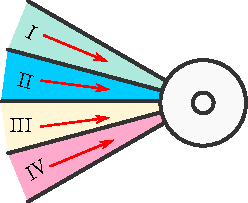
\includegraphics[width=0.9\linewidth]{figures/anti-aircraft.pdf}
\caption{Strategies with aeroplanes and anti-aircraft guns.\label{anti-aircraft}}
%fig 2.14
 \end{wrapfigure}

\txthead{Airplanes against antiaircraft guns.} Let us find the optimal mixed
strategy for a concrete game. Suppose ``player'' $A$ wants to attack
``player'' $B$. $A$ has two airplanes each carrying a large bomb. $B$ has four
antiaircraft guns defending an important military base. To destroy the
base, it is sufficient for at least one airplane to approach it. To approach
the base the airplanes may choose one of four air corridors (\figr{anti-aircraft}, where 0 is the base and I, II, III, and IV are the air corridors). $A$ may send both airplanes along the same corridor or along different corridors. $B$ may place his four antiaircraft guns to cover the corridors in different ways. Each gun can only shoot once, but it will hit the airplane if it is in that corridor.
 
$A$ has two pure strategies: strategy $A_{1}$ to send the airplanes along
different corridors (no matter which ones), and $A_{2}$, to send both
airplanes along the same corridor. $B$'s strategies are $B_{1}$ to put an
antiaircraft gun into each corridor, $B_{2}$ to put two guns into two
corridors (leaving the other two corridors unprotected), $B_{3}$ to put two
guns into one corridor and one gun into two of the other corridors, $B_{4}$
to put three guns into a corridor and one gun into another corridor,
and $B_{5}$ to put all four guns into one corridor. Strategies $B_{4}$ and $B_{5}$ are certainly bad because three or four guns in a single corridor are not
needed, since $A$ only has two airplanes. Therefore, we need only discuss
strategies $B_{1}$, $B_{2}$, and $B_{3}$.

 \begin{wrapfigure}{O}{\mfwidth}
 \centering
 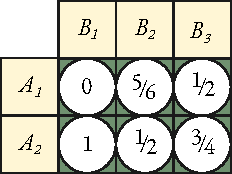
\includegraphics[width=0.7\linewidth]{figures/aa-matrix.pdf}
\caption{Matrix of probable with aeroplanes and anti-aircraft guns.\label{aa-matrix}}
%fig 2.15
 \end{wrapfigure}
Suppose $A$ chooses strategy $A_{1}$ and $B$ chooses strategy $B_{1}$. It is clear that neither airplane will reach base: the $A$'s gain will be zero ($a_{11}=0$). Suppose strategies $A_{1}$ and $B_{2}$ are chosen. Let us assume that the guns are in corridors I and II. If the aircrafts are flying along different corridors, then six variants are equally probable: they fly along corridors I and II, along corridors I and III, along corridors I and IV, along II and III, along II and IV, or along III and IV. In only one of the six cases will neither plane reach the base (when they fly along corridors I and II). Whichever corridor $B$ chooses to place his guns in, airplanes will always have six equally probable variants and only one does not yield a winning move. Therefore, if strategies $A_{1}$ and 
$B_{2}$ are chosen, the probable gain for $A$ will be 5/6 ($a_{12}$ = 5/6). Reasoning in the same manner, it is easy to find the rest of the elements of the
payoff matrix for this game. The resultant $2 \times 3$ matrix is shown in
\figr{aa-matrix}. Note that the elements of the matrix are \redem{probable} gains; so here even the pure strategies involve chance. The lower value of the
game is 1/2, and the upper one is 3/4. The maximin strategy is $A_{2}$ while
the minimax strategy is $B_{3}$. There is no saddle point, and the optimal
solution for the game will be a mixed strategy.

In order to find the optimal mixed strategy, let us use the payoff
matrix and relations \eqref{eq-2.12} and \eqref{eq-2.13}. The relations for this case are
\begin{align}%
 x_{2} \geqslant 1, \quad \frac{5}{6}x_{1} + \frac{1}{2} x_{2}  \geqslant 1, \quad  \frac{1}{2}x_{1} + \frac{3}{4} x_{2} & \geqslant 1 \label{eq-2.14},\\
x_{1} + x_{2} & = \frac{1}{\nu}. \label{eq-2.15}
\end{align}
The solution can be conveniently represented as a diagram. We plot
the positive values $x_{1}$ and $x_{2}$ along the coordinate axes (\figr{aa-graph}). The first inequality in \eqref{eq-2.14} corresponds to the area above the straight line $CC$; the second inequality is the area above $DD$; and the third inequality in \eqref{eq-2.14} is the area above $EE$. All three inequalities are satisfied inside the area shaded red in the figure. The equation $x_{1} + x_{2} = \text{const}$ defines a family of straight lines, some of which are shown in figure as dash lines. The straight line $FF$ has the least sum $x_{1} + x_{2}$ of all the lines in the family with at least one point within the red area. Point
$G$ indicates the solution corresponding to the \redem{optimal mixed strategy}.
The coordinates of this point are  $x_{1} = 3/5$ and  $x_{2} = 1$. Hence we find
$\nu = 5/8, \, p_{1} = 3/8, \, \text{and} \, p_{2} = 5/8$. Thus, $A$'s optimal mixed strategy would be to use strategy $A_{1}$ with probability 3/8 and strategy $A_{2}$ with probability 5/8.
 \begin{figure}[!h]
 \centering
 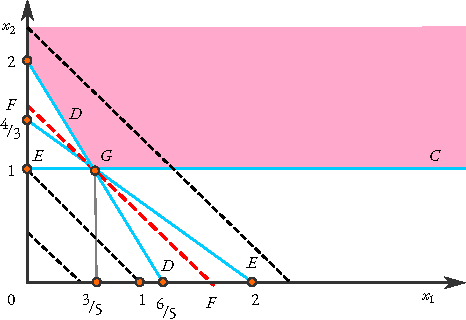
\includegraphics[width=0.85\tfwidth]{figures/aa-graph.pdf}
\caption{Solution for the game of aircrafts and anti-aircraft guns.\label{aa-graph}}
%fig 2.16
 \end{figure}

How could we use this recommendation in practice? If there is only
\redem{one} bombing raid in the ``game''. A clearly should select strategy $A_{2}$ because $p_{2} > p_{1}$. Suppose now the game has \redem{many} raids (for instance, raids on many bases). If the game is run $N$ times ($N \gg 1$), then $A$ should choose strategy $A_{1} \,\, 3N/8$ times and strategy $A_{2} \,\, 5N/8$ times.

We have so far only discussed the behaviour of $A$, allowing $B$ to act
arbitrarily. If $A$ selects his optimal mixed strategy, his average gain will
be between the upper game value of 3/4 and the game value $\nu = 5/8$. If
$B$ behaves unreasonably, the $A$'s gain may rise to the upper value of the
game (or even greater). However, if $B$ in turn adheres to his optimal
mixed strategy, the $A$'s gain will equal the game value $\nu$. The optimal
mixed strategy for $B$ precludes his use of strategy $B_{3}$ and is to use
strategy $B_{1}$ with probability 1/4 and strategy $B_{2}$ with probability 3/4.
That strategy $B_{3}$ should not be used can be seen from \figr{aa-graph}: the
straight line $EE$ corresponding to this strategy does not have any points
in the red area. To determine the probabilities with which to apply
strategies $B_{1}$  and $B_{2}$, we use the game value $\nu = 5/8$, and get $q_{1} \times 0 + (1 - q_{1}) \times 5/6 = 5/8$. It is clear from this that $q_{1} = 1/4$ and $q_{2} = 1 - q_{1} = 3/4$.

% \upsilon can be used instead of \nu

%%% Local Variables:
%%% mode: latex
%%% TeX-engine: xetex
%%% TeX-master: "twibop2"
%%% End:
